\section{Method}
In this section, we explore different self-supervised approaches to leverage the benefits of self-supervised learning: we adopt the image-based DINO \cite{caron2021emerging} approach for 3D skeleton data and combine this SkeletonDINO with SkeletonBT \cite{zhou2023self} to our proposed SkelDINO-SAM. 

\subsection{SkeletonDINO}
In our adaptation inspired by DINO \cite{caron2021emerging}, we leverage its self-distillation framework to enhance label-free skeleton-based action recognition. 
Similar to the original DINO concept, our approach employs two encoder models: the student and the teacher network. The primary objective remains for the student to learn robust representations guided by the teacher. Central to this technique is self-distillation, where the teacher network guides the learning process of the student network through cross-entropy loss.

By processing two different random transformations of an input, akin to the approach in DINO with image data, we pass two skeleton sequences through both the student network ($g_{\theta_s}$) with parameters $\theta_s$ and the teacher ($g_{\theta_t}$) network with parameters $\theta_t$. Each network produces a $K$-dimensional feature representation, denoted as $P_s$ and $P_t$, respectively.

To ensure stable and effective learning, these feature representations undergo normalization using softmax operations with temperature parameters, $\tau_s$ for the student and $\tau_t$ for the teacher. This normalization step maintains the features within a desired range for learning and generalization:

\begin{center}
$P_s(x)^{(i)}=\frac{\exp \left(g_{\theta_s}(x)^{(i)} / \tau_s\right)}{\sum_{k=1}^K \exp \left(g_{\theta_s}(x)^{(k)} / \tau_s\right)}$,
\end{center}

The core of the DINO framework lies in the self-distillation process. The teacher is not updated during  back propagation only the weights of the student network are updated based on the cross-entropy loss:

\begin{center}
$\min _{\theta_s} H\left(P_t(x), P_s(x)\right)$
\end{center}

where:

\begin{center}
$H(a, b)=-a \log b$
\end{center}

The aim is to maximise similarity between the student and teacher features by minimizing the cross-entropy loss. A original skeleton sequence $x$ and a noisy augmentation $x_n$ of the original skeleton sequence are passed to both networks. Only the student network receives masked augmentations. Specifically, given a skeleton sequence and a set $V$ of different skeleton augmentations, the loss function is defined to minimize the cross-entropy between the teacher and student features:

$$
\min _{\theta_s} \sum_{x \in\left\{x_1^g, x_2^g\right\}} \sum_{\substack{x^{\prime} \in V \\ x^{\prime} \neq x}} H\left(P_t(x), P_s\left(x^{\prime}\right)\right)
$$

This loss function drives the student to learn meaningful and discriminativ representations by mimicking the knowledge present in the teacher's feature space. A crucial aspect of DINO is the use of exponential moving average (EMA) to update the teacher parameters $\theta_t$. The teacher network learns from the EMA of the student network parameters, resulting in smoother and more consistent updates. This technique stabilizes the learning process and helps the student converge to meaningful representations. 

%The neural network $g$ is composed of a backbone $f$ which is the STTFormer, and a projection head $h$: $g=h\circ f$. The features used in downstream tasks are the backbone $f$ outputs. The projection head comprises of two layers of a multi-layer perceptron (MLP) with a hidden dimension of 512, l2 normalization, and a fully connected layer (Weight Norm) with weight normalization and K dimensions.

Centering \cite{caron2021emerging} is used to prevent one dimension from dominating while encouraging collapse to a uniform distribution, whereas sharpening \cite{caron2021emerging} does the reverse. The use of both processes balances the impact they have. Output sharpening is carried out by setting the temperature $\tau_t$ to a low value in the teacher's softmax normalization. 
This mechanism has been proven to have a similar impact as the negative samples \cite{caron2021emerging} in which it makes the system learn meaningful representations and prevent collapsing to a uniform distribution. 

\subsection{Separated Augmentation Modules}

For the implementation of the separated augmentation modules (SAM) we first adopt weighted masking according to \textcite{zhou2023self}. The process of assigning masked probabilities is as follows: Let \(V_i\) denote the \(i\)-th joint in the skeleton, where \(i \in (1, 2, ..., n)\), and \(n\) is the total number of joints in the skeleton. .

To calculate the masked probability for each joint \(V_i\), the degree \(d_i\) of each joint is first computed, and then the probability \(p_i\) is set as follows:

\[ p_i = \frac{d_i}{\sum_{j=1}^n d_j} \]

where \(d_i\) represents the degree of the \(i\)-th joint, and the denominator \(\sum_{j=1}^n d_j\) ensures that the probabilities are normalized to 1. By using this Central Spatial Masking (CSM)~\cite{zhou2023self}, we focus on masking joints based on their degree centrality, enhancing the encoder's ability to capture a broader range of joint relationships.

In the temporal masking stream, the Motion Attention Temporal Masking (MATM)~\cite{zhou2023self} strategy is introduced to prioritize frames that change quickly. These frames often contain more semantic information about the actions, making them more valuable for learning meaningful representations. To compute the motion \(m \in \mathbb{R}^{C \times T \times V}\) of the sequences, the temporal displacement between frames is calculated as \(m_{:,t,:} = x_{:,t+1,:} - x_{:,t,:}\), where \(x_{:,t,:}\) and \(t\) is the index of the frame.

Next, MATM calculates the overall motion rate of a frame, which serves as the attention weight. The motion rate \(a_t\) for frame \(t\) is computed as follows:

\[ a_t = \frac{(m_t)^2}{\sum_{i=1}^T (m_i)^2} \]

where \(a_t\) represents the motion rate of frame \(t\), and the denominator \(\sum_{i=1}^T (m_i)^2\) ensures that the attention weights are normalized to 1.

Once the attention weights are computed, the top-K attention weights \(a_{t1}, ..., a_{t_K}\) are selected, and the corresponding frames \(x_{t_1}, ..., x_{t_K}\) serve as the key-frames that contain more semantic information about the actions. These key-frames are then masked, and the encoder is encouraged to capture the relationship between the feature from the masked sequence and the anchor feature, which contains the total semantic information.

\begin{figure}[t]
      \centering
      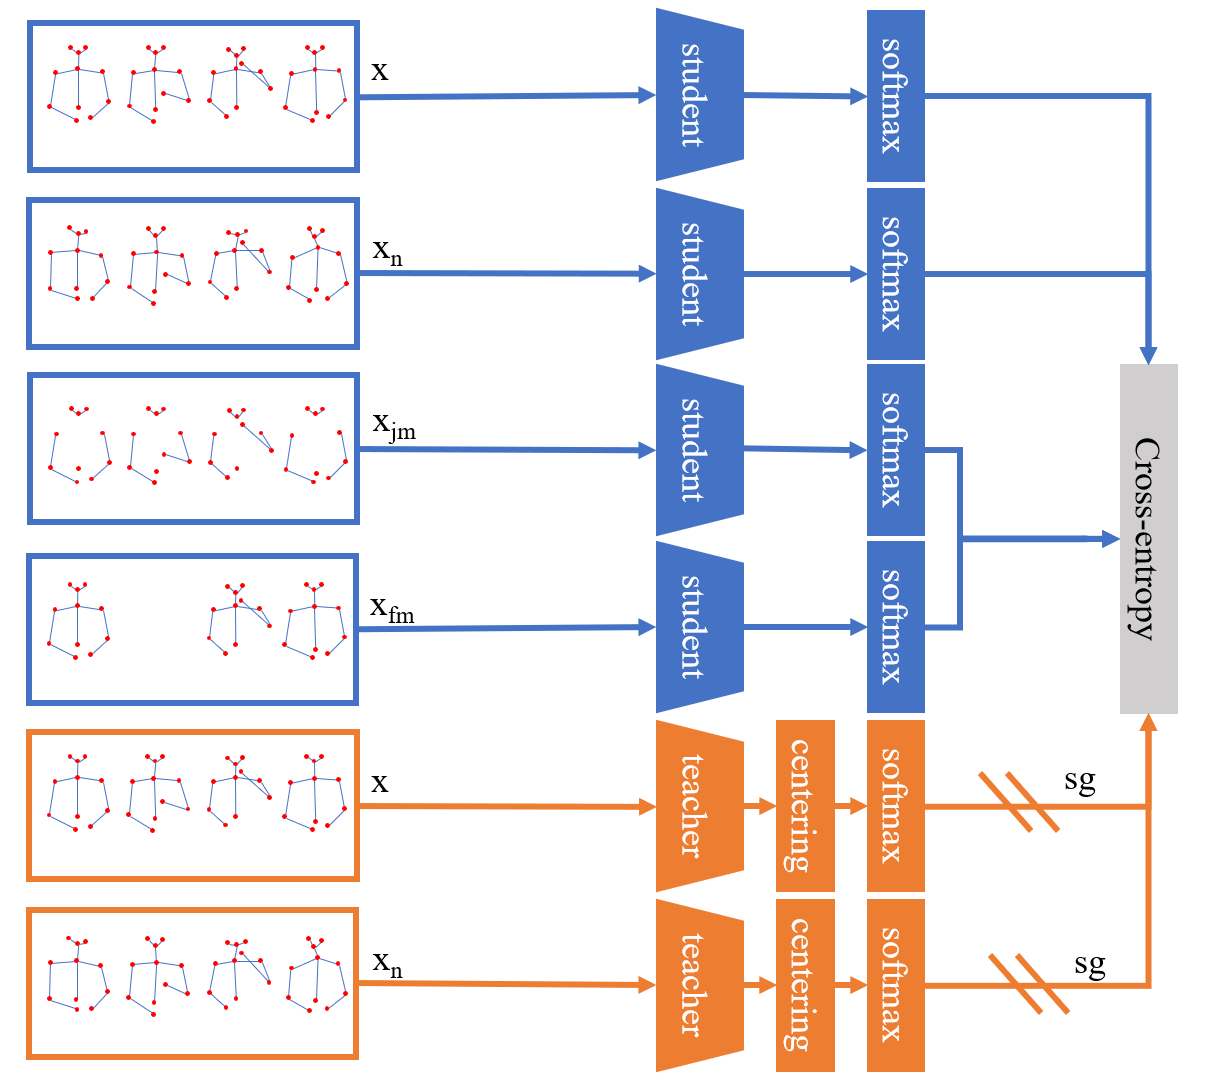
\includegraphics[width=\linewidth]{figures/principle.png}
      \caption{Principle of our SkelDINO-SAM approach. It consists of a student (blue) and a teacher network (orange). The student network receives the original skeleton sequence $x$ and the augmentation with additive noise $x_n$ as well as the frame masked $x_{fm}$ and joint masked sequence $x_{jm}$. The teacher network receives the original skeleton sequence $x$ and the augmentation with additive noise $x_n$.}
      \label{fig:principle}
\end{figure}

\subsection{SkeletonDINO with SAM}
In our SkeletonDINO with SAM (SkelDINO-SAM, see Figure~\ref{fig:principle}), we introduce a novel approach that combines the principles of SkeletonDINO with the concept of SAM, inspired by the work of \textcite{zhou2023self}. Unlike images, skeleton representations are inherently more concise, making them particularly amenable to targeted augmentation strategies. As such, we opt to employ distinct augmentation pipelines for different aspects of the skeleton sequence, rather than applying random augmentations uniformly across the entire sequence.

This approach results in the creation of four distinct inputs for the student network. In addition to the original skeleton sequence, the student network receives variations of the input data, including sequences with additive noise and sequences with joint and frame masking. By diversifying the input data in this manner, we aim to enrich the learning process and enable the student network to better generalize across different types of noise and occlusions.
%For the teacher network input, we adopt a similar strategy, providing both the original sequence and a version with additive noise. This ensures that the teacher network is equipped with diverse training data, allowing it to effectively guide the learning process of the student network while also promoting robustness to various sources of noise and perturbations in the input data.
In the proposed method, the teacher model receives two distinct sets of input data the original skeleton sequence $x$ and the noisy sequence $x_n$. These inputs are embedded by the teacher model. The teacher output embeddings are then centered \cite{caron2021emerging}.

Concurrently, the student model processes multiple sets of input data, including the original skeleton sequence $x$ and the sequence with additive noise $x_n$ as well as the frame masked sequence $x_{fm}$ and the joint masked sequence $x_{jm}$. Each set of data undergoes independent processing within the student model, followed by the application of a softmax function akin to the teacher model. The objective involves comparing the outputs of both teacher and student models using a cross-entropy loss function. Through minimizing this loss, the student model endeavors to approximate the behavior of the teacher model.

%\pagebreak